% !TEX root = thesis.tex
This chapter's purpose is to give context to the Advanced Encryption Standard (\ac{AES}) algorithm. It starts with a brief history of digital cryptography, explains the \ac{AES}-selection-process and then gives some examples of security issues that have been found over the years.


\section{Before AES}
\label{ch:before-aes}
The progress made in the field of information technologies during the second half of the 20th century did affect large areas of our society. Amongst others it massively influenced cryptography. \cite{cryptorebels} illustrates how the ever increasing availability of computers made rapid advancements in cryptography possible. First digital computation provided the basis for a new encryption scheme, devised in 1975 by Winfried Diffie and Martin Hellman, called public-key cryptography. This solved an old problem in cryptography, namely establishing a shared secret over an insecure communication channel. Previous encryption schemes always relied on such a secret, like a password, that needs exchanging between the communicating parties, before messages can be en- and decrypted with this password. Since public-key cryptography encrypts and decrypts with two different keys, communicating parties are able to simply exchange their encryption keys over an insecure channel. As long as both parties keep their decryption keys private they can exchange messages securely by using each others encryption key to prepare messages for transit.
The first openly available standard for electronic encryption was a symmetric cipher called "Data Encryption Standard" or DES (\cite[p. 105]{appcrypt}. Developed in the early 1970s at IBM after a request from the National Bureau of Standards (which later on became \ac{NIST}) the cipher was published in 1977 as an official Federal Information Processing Standard (\ac{FIPS}). For \cite[p. 2]{cryptodream} DES and the public-key encryption scheme with the algorithms RSA and the Diffie-Hellman key exchange derived from it, represented a fundamental shift in the field of cryptography. Before the fight between coders and code breakers seemed to always go in favour of the party with superior skill and resource. Suddenly, at the end of the seventies, encryption for everyone, proven secure by mathematics seemed within reach for wide parts of the populations. In the foreseeable future even modest computing resources would be able to apply algorithms to plaintext, that could render it undecipherable, even for adversaries with the skills and resources of entire governments supporting them. For the first time not even knowledge of cryptography was needed to secure messages, since once implemented, everyone able to execute the algorithm could use it to encrypt.

The security of DES was widely disputed though. Even in the late seventies the key length was criticized as too short, provoking speculation about \ac{US} intelligence agencies applying pressure to intentionally weaken the algorithm, although it took until June of 1997 before the first DES message was publicly decrypted via brute force attack (\cite[p.112]{appcrypt}). \footnote{As of February 2021 crack.sh claims "to achieve an average crack time of 25 seconds and a success rate of 99.5\%" for any DES-key.} In January of the same year the search for a predecessor of DES was announced by the National Institute of Standards and Technology of the United States (NIST). This predecessor supposed to be "an unclassified, publicly disclosed encryption algorithm capable of protecting sensitive government information well into the next century."\cite[p. 1]{announcementrequest}.To increase trust into this standard-to-be the search was public and \ac{NIST} relied on submissions from the cryptographic community.
This openness in competition combined with a total lack of usage restrictions in- and outside the \ac{US} represented a massive shift in the United States governments stance on cryptography. 
Since the late seventies government agencies like the \ac{NSA} openly advocated against "unrestrained public discussion of cryptologic matters", even going as far as trying to suppress the scientific discourse. (\cite[p. 151-152]{cyberhist}). For a time the export of cryptographic devices and software from the \ac{US} to other countries was placed under the International Traffic in Arms Regulations \cite[Category XIII--Auxiliary Military Equipment $(1)$]{armslaw} . This changed only when the \ac{AES} competition was well underway (\cite{revisedlaw}).

\section{The Advanced Encryption Standard selection}
\label{ch:aes-selection}

The following chapter is, if not mentioned otherwise, based on \cite{nistdevoverview}.

The formal call for submissions of \ac{AES} candidates came in September of 1997. \ac{NIST} explicitly requested input from outside of the institution by explicitly asking \enquote{the public, academic/research communities, manufacturers, voluntary standards organizations, and Federal, state, and local government organizations.} The submissions would be made public for review and comment after the submission period

\subsection{Requirements}
\label{ch:requirements}

The proposed algorithms for the new encryption standard and thus the
potential successors of DES had to fulfill a number of requirements, as can be found in \cite{announcementrequest}, in order for them to be considered by \ac{NIST}. \ac{AES} was intended to be a block cipher operating on 128 bits at a time. Those bits should be secured by
key length of at least the three sizes 128, 192 and 256 bits.
The candidates would be furthermore analyzed and evaluated regarding:

\begin{itemize}
\item
  \emph{security}: Deemed as the most important criterion, it
  encompasses factors like the actual security compared to the
  competitors, the degree to which the algorithm is able to produce an
  output indistinguishable to a random permutation of the input, the
  quality of the mathematical principles behind the algorithm and of
  course critique, concerns and attacks regarding the candidates
  originating from the public review.
\item
  \emph{cost}: Financial cost was one consideration: All candidates had
  to be released on a ``worldwide, non-exclusive, royalty-free basis.''
  before they could be submitted. Performance costs like the speed of
  the algorithm both in software and hardware implementations or memory
  size, be it in code size, gate count for hardware implementations or
  RAM requirements for software implementations were further factors
  that played a role in this category.
\item
  \emph{algorithm and implementation characteristics}: Flexibility
  without compromising security was another desirable aspect of the new
  standard. Additional key sizes to those specified in the minimum
  requirements, the possibility of implementation on a variety of
  platforms, from slower 8-bit SmartCard processors to fully-fledged
  desktop CPUs and other fields of applications like usage as a stream
  cipher, message authentication generator, pseudorandom number
  generator, hashing algorithm and more were all attributes to the
  flexibility of an encryption algorithm an thus factors, that
  influenced the \ac{AES}-committee in their final decision. The last aspect
  under which the standard-to-be had to prove itself was simplicity,
  where a simpler algorithm, that holds up well under all other aspects,
  is preferable.
\end{itemize}


\subsection{The \ac{AES} selection process}
\label{ch:aes}

\begin{figure}
  \centering
  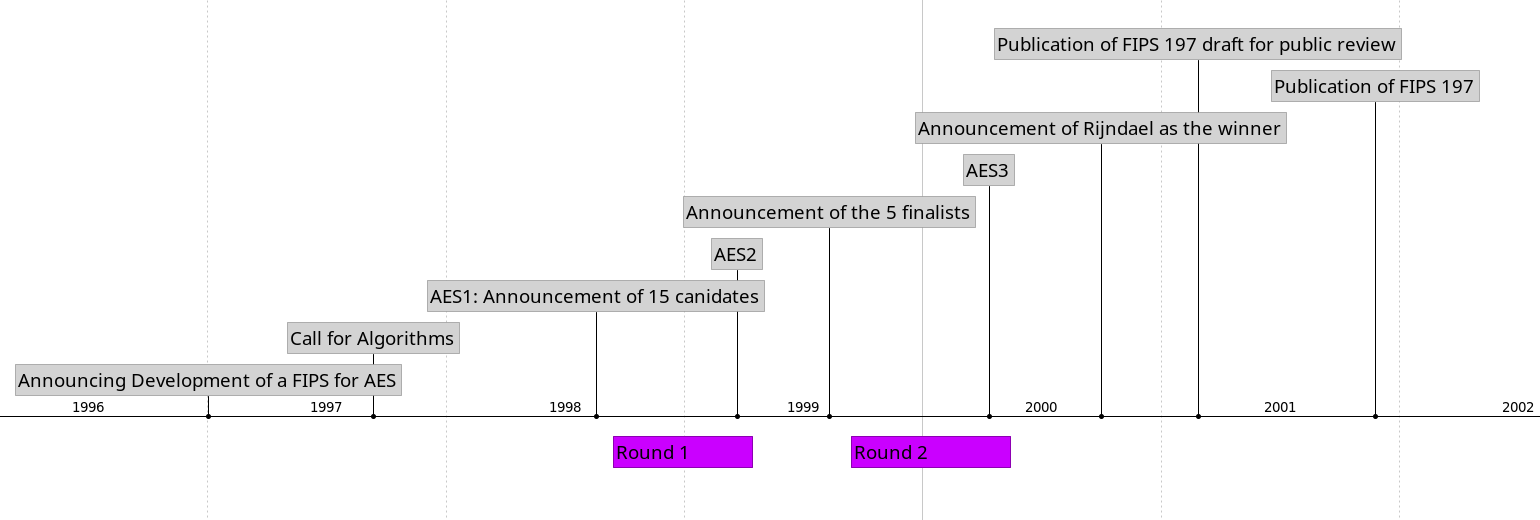
\includegraphics[scale=0.37]{data/figures/aes-process-timeline.png}
  \caption{Notable events in the \ac{AES} selection process}
  \label{fig:procestimeline}
\end{figure}

Nearly a year after requesting submissions, \ac{NIST} published a list with fifteen candidates they deemed worthy of further investigation at the First \ac{AES} Candidate Conference (AES1) in August 1998. The cryptographic community was invited to critique those choices, either via email or later on in the online discussion forum \ac{NIST} hosted for this exact purpose. This input from the community collected in "Round 1" of the selection process was discussed at the Second \ac{AES} Candidate Conference (AES2) in spring of 1999. Shortly after that \ac{NIST} selected in their publication \cite{round1report} five finalists from the initial fifteen algorithms: MARS, RC6, Rijndael, Serpent, and Twofish.
The other candidates were excluded, partially because "serious questions [had] been raised about [their] security" (p.34), partially because they were slower/potentially less secure than other comparable candidates.
The finalists moved on to receive further scrutiny from both the \ac{NIST} and the cryptographic community in the so called "Round 2".
After this more in-depth analysis of the algorithms a third conference (AES2) in April 2000 provided an open, public forum to review and discuss the findings accumulated up to this point in Round 2. The authors of the finalists were explicitly invited to partake in the process. A month later Round 2 came to an end and \ac{NIST} moved on to select the algorithm they deemed to be best suited as the new Advanced Encryption Standard.
On October of the same year the institute announced in \cite{round2report} their decision to propose Rijndael, authored by Joan Daemen and Vincent Rijmen, as the \ac{AES}. Each finalist "appears  to  offer adequate security, and each offers a considerable number of advantages" (p.91), but "Rijndael’s combination of security, performance, efficiency, implementability, and flexibility make it an appropriate selection for the AES" (p.92).
The proposal was formalized in a \ac{FIPS} draft for the Advanced Encryption Standard and published on February 2001 (\cite{fipsdraft}). After going through the usual \ac{FIPS}-approval-process the Advanced Encryption Standard was made public as \ac{FIPS} 197 \cite{fips197} at the end of the year.

\section{AES in review}
\label{ch:aes-review}

The slightly modified Rijndael that is known as \ac{AES} today has been subject to a lot of analysis over the years, with many focusing on the security aspects of the algorithm. The following selection of literature is a selection and does not claim complete coverage of the subject.

\subsection{NIST}
\label{ch:nist-review}

From their Round-2-Report \cite{round2report} can gain some insight in how \ac{NIST} thought about Rijndael in detail.
Although they acknowledged that some voiced criticism regarding its mathematical structure offering a potential attack vector on the algorithm, they believe that the simplicity of said structure facilitated a deeper understanding of the security properties Rijndael brings to the table. Overall they report to have no knowledge of a security attack against Rijndael.
The good performance of the algorithm under a variety of circumstances is emphasised, be it 8- or 64-bit software implementations, as well as the ease, with which the algorithm is able to run in an parallel setup, the fast key setup time, low memory and disk space footprints and the speed of the hardware implementation.
\ac{NIST} states that Rijndael is -thanks to its operations used- one of the easiest algorithms of the finalist to defend against power and timing side-channel attacks. The institute did not notice a great hit in performance while testing a hardened version of Rijndael, at least in comparison to the other finalists. Some power analysis attacks still seem to be effective though, even with the hardened Rijndael.
Key setup time and key agility were two other strong areas for Rijndael in the eyes of \ac{NIST}. Furthermore the authors hint at the possibility of flexible key and block sizes, which, while not really considered at the time of the report, is seen as another sign in favor of Rijndael.

\subsection{Side Channel Attacks}
\label{ch:sidechannelattacks}

The cryptographer Bernstein described in \cite{bernsteincache} a successful key-extraction via network from the OpenSSL \ac{AES} implementation running on a Pentium III (both very common software and hardware at the time). This side-channel attack was in his eyes not a result of a faulty implementation, but an inherent flaw in the design of the algorithm that makes it "extremely difficult to write constant-time high-speed \ac{AES} software for common general-purpose CPUs." (p.1). In many cases Bernstein can make out a correlation between the time it takes to load an array entry and the index of an entry in said array. Thus the time it takes to load an entry leaks information about the information currently processed within the algorithm ultimately revealing the key to an attacker, if said attacker can piece the leaked information together in the right way.
According to Bernstein, this is not only a problem inherent to \ac{AES}, but to all cryptographic algorithm implementations that rely heavily on lookup tables to speed up their computation.
Joseph Bonneau and Ilya Mironov state in a conference paper from 2006  \cite{improvedcache}, that while Bernstein's "approach is widely applicable" (p.205), it is far from ideal, as it needs timing data from approximately $2^{27.5}$ encrypted samples. Furthermore the fragility of the Bernstein's attack is one of the main drawbacks according to the authors. The attacker needs to replicate the targeted machine with a lot of care, since small differences between target and replication will produce unusable timing data, leading to failure of the attack. Their own cache-collision timing attacks -while being orders of magnitude faster under optimal circumstances than the previously discussed attack- are representing "a significant step towards developing realistic remote timing attacks against AES" (p.210).
The power draw of the encrypting CPU seems to represent another attack vector on the algorithm. In \cite{powerdraw} the authors force the eviction of selected parts of \ac{AES} lookup tables and measure the increased power draw from the CPU in case of a cache miss in the following encryption calculations. With that the authors claim to be able to extract the complete secret key. While the attack itself is described as "quite simple" (p.6), the same statement is made for the proposed countermeasure.
\cite{ctattacksfeasible} finds that the ease of \ac{AES}-cache-behavior exploitation is not necessarily true anymore on more modern x86-processors. Features like multiple cores per processor with each having its own cache, the increased cache pressure emitted from more complex software, physically tagged caches, the partially undocumented, and very complex prefetcher units, and of course the \ac{AES-NI} instruction set make it "substantially more difficult to mount data-cache side-channel attacks on \ac{AES} than previously realized." (p.1). As in \cite{aes-ni} stated, \ac{AES-NI} itself promises to prevent some software side-channel attacks single-handedly by sheer virtue of not having to use lookup tables for a fast implementation of the encryption algorithm.
This does not necessarily apply to the slew of novel attacks categorized as 'transient execution CPU vulnerabilities' (see \cite{transientexecution}), but since they do not target \ac{AES} directly they will not be discussed here.

\subsection{Mathematical Attacks}
\label{ch:mathematicalattacks}

During the \ac{AES} development the first papers with attacks on Rijndael were published. \cite{Gilbert00acollision} demonstrated an attack that broke seven rounds of \ac{AES} with any key length, but the attacks "complexity is very high even if the number of plaintexts to cipher is small." (p.11). The authors did not see a danger to the complete 10-round-version.
Roughly around the same time \cite{impcryptan} published and attack, that managed to break one round more for each AES-192 and AES-256, but "[m]any of these attacks require virtually the entire codebook of texts and hence are not very practical." (p.15).
The key schedule of Rijndael was criticized in the same paper, the authors found it "worrisome" (p.15). \cite{rkeyattack} expressed similar concerns, even going as far as labeling it as weak, since it was for example enabling related-key attacks on the full rounds of AES-192 and AES-256 algorithm, which the authors found out earlier in \cite{rkeyattack2}.  While those attacks "are still mainly of theoretical interest [at the time] and do not present a threat to practical applications using AES" (p.14), or related-key attacks in general are not " not universally accepted as a practical attack model."\cite[p. 14]{rkeyattack3} they also "should not be possible in a good cipher." \cite{rkeyattack} (p.13).
\cite{rkeyattack3} continues chipping away at the confidence held in the 256-bit variant of \ac{AES}, describing key derivation attacks "of practical complexity" (p.2) on a 10-round variant of that algorithm. The authors identify again the design of the key-schedule as a culprit, which they deem "not of industrial strength" (p.14). The attack seems ineffective against the 128-bit variant of the encryption algorithm. Nevertheless the authors are of the opinion, that "AES can no longer be considered as a safe black box construction, which can be dropped into any security application with little thought about how it is used.", a notion, which they think of as "disturbing"(p.14).
One of the most successful attacks on the algorithm was described in \cite{biclique} where the authors used Biclique Cryptanalysis to mount a better-than-brute-force-attack on \ac{AES} with all rounds used as described in the standard, effectively reducing the key strength of each \ac{AES} variant by a few bits. But even with this novel approach it still remains infeasible to recover a \ac{AES}-encrypted plaintext from a ciphertext without the key or usage of side channels.



